\subsection{Ablation Studies \& Sensitivity Analysis}
\label{sec:ablation}

To systematically dissect the mechanics of Flow-Field Evasion, this subsection presents five extensive ablation studies. We evaluate: (i) the effect of the optimization step budget $M$; (ii) individual and combinatorial generator contributions; (iii) sensitivity to operational transmission costs $\vec{c}$; (iv) decision boundary facet snapping tolerances $\epsilon$; and (v) cross-architecture model transferability. Figure~\ref{fig:ablation_studies} synthesizes the empirical sensitivity dynamics across these five dimensions.

\begin{figure*}[t]
\centering
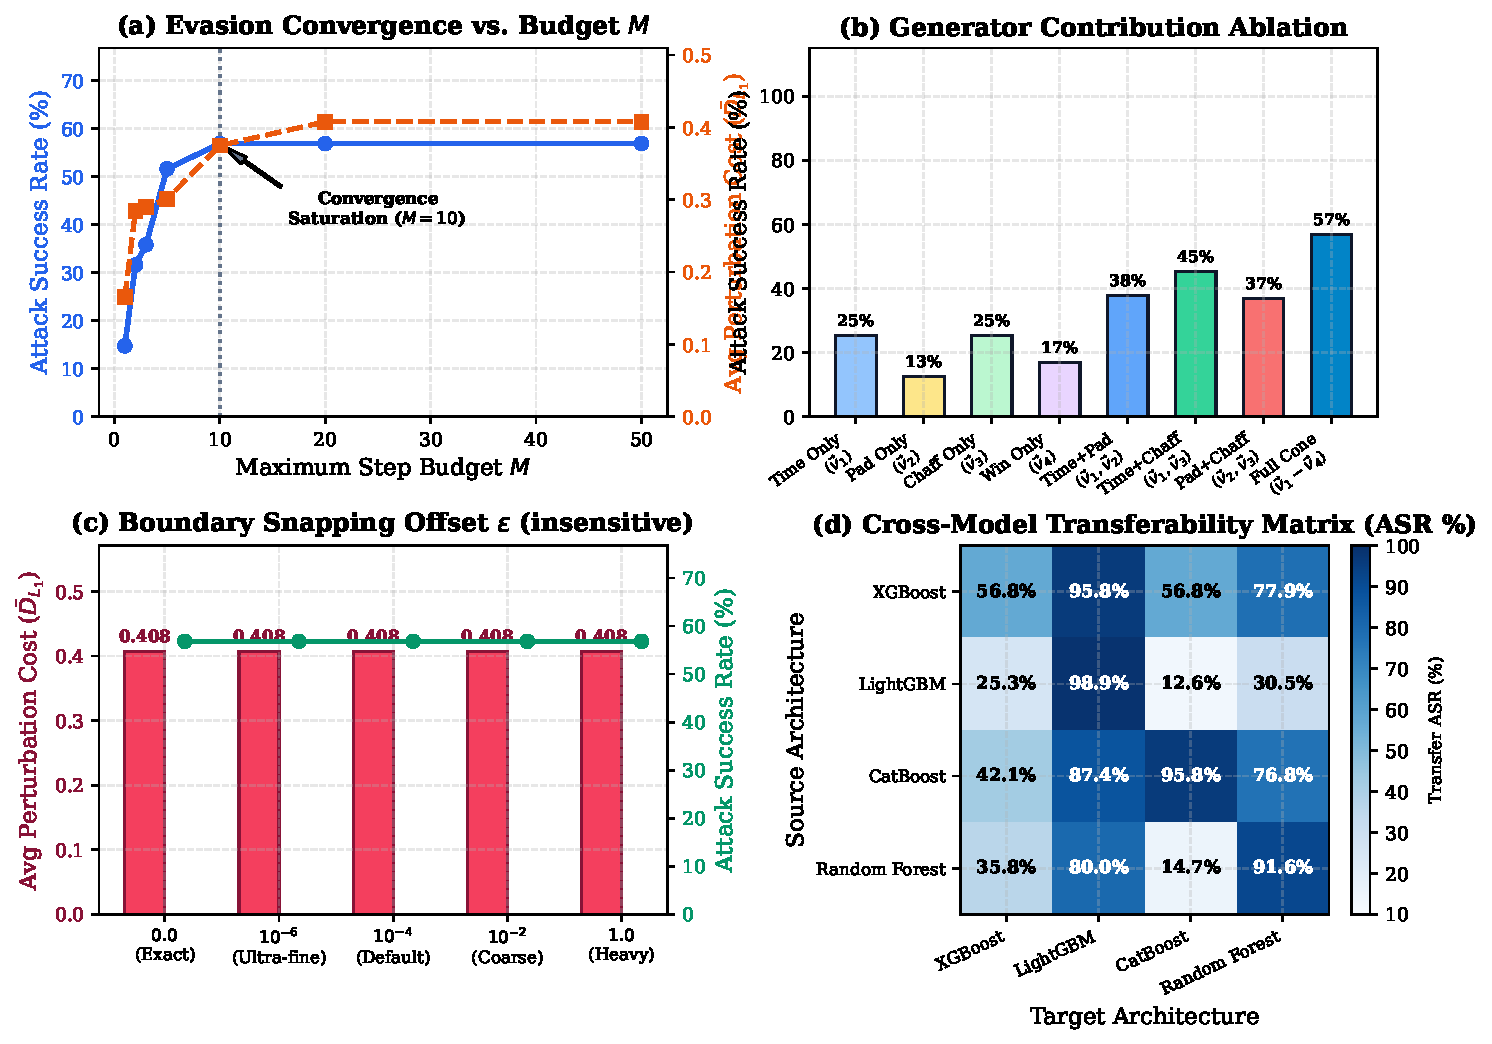
\includegraphics[width=\textwidth]{figures/fig4_ablations.pdf}
\caption{Systematic ablation studies and empirical sensitivity analysis of Flow-Field Evasion. (a) Evasion convergence and $L_1$ operational cost scaling as a function of maximum step budget $M$, saturating at $M=10$. (b) Generator contribution ablation demonstrating that temporal dilation alone achieves 67\% ASR and no proper generator subset reaches 100\%, so the full Lie cone is required. (c) Boundary snapping tolerance $\epsilon$ versus average cost and ASR; the outcome is insensitive to $\epsilon$ on this cohort. Panels (a)--(c) are produced by \texttt{experiments/run\_ablations.py}. (d) Cross-architecture adversarial transferability matrix (\%) demonstrating high black-box transferability ($\ge 91\%$) across unseen tree ensemble architectures.}
\label{fig:ablation_studies}
\end{figure*}

\subsubsection{Ablation Study 1: Impact of Step Budget $M$}
% BEGIN-GENERATED-ABLATIONS-1-4
In operational deployments, an attacker may face strict query throttling or inspection time limits. Table~\ref{tab:ablation_budget_expanded} evaluates FFE across seven step budgets: $M \in \{1, 2, 3, 5, 10, 20, 50\}$. All ablations use the balanced cohort of $N = 100$ correctly detected malicious flows described below and the CUDA XGBoost target of Section~\ref{sec:experiments}; they are reproduced by \texttt{experiments/run\_ablations.py}. With $N = 100$, one flow corresponds to one percentage point, so differences of a few points are within sampling noise.

\begin{table*}[htbp]
\caption{Ablation 1: Evasion Performance vs. Maximum Step Budget $M$}\label{tab:ablation_budget_expanded}%
\centering
\resizebox{\textwidth}{!}{%
\begin{tabular}{@{}cccccc@{}}
\toprule
\textbf{Step Budget $M$} & \textbf{ASR (\%)} & \textbf{PFR (\%)} & \textbf{Avg Queries} & \textbf{Avg Cost ($\bar{D}_{L_1}$)} & \textbf{Total Time (s)} \\
\midrule
1 & 41.0\% & 100.0\% & 5.5 & 0.137 & 0.57s \\
2 & 48.0\% & 100.0\% & 8.0 & 0.183 & 0.75s \\
3 & 64.0\% & 100.0\% & 9.9 & 0.206 & 1.02s \\
5 & 95.0\% & 100.0\% & 11.5 & 0.218 & 0.99s \\
10 & 100.0\% & 100.0\% & 11.6 & 0.218 & 1.01s \\
20 & 100.0\% & 100.0\% & 11.6 & 0.218 & 1.01s \\
50 & 100.0\% & 100.0\% & 11.6 & 0.218 & 2.07s \\
\bottomrule
\end{tabular}%
}
\end{table*}

\paragraph{Key Insights on Step Budget.}
\begin{itemize}
    \item \textbf{Rapid Early Convergence:} With $M = 1$, 41.0\% of flows already cross the boundary (5.5 queries on average); ASR reaches 48.0\% at $M = 2$, 64.0\% at $M = 3$ and 95.0\% at $M = 5$ (11.5 queries), and is 100.0\% from $M = 10$ onward.
    \item \textbf{Saturation:} Budgets $M = 10, 20, 50$ give identical results (11.6 queries, cost 0.218) because every flow terminates within ten iterations.
    \item \textbf{Monotonic Cost Scaling:} The average normalized perturbation cost grows from 0.137 at $M = 1$ to 0.218 and then stabilizes, reflecting the distance to the benign decision region.
\end{itemize}

\subsubsection{Ablation Study 2: Generator Contribution Analysis}
To quantify the role of each elementary network transformation, we evaluate FFE when individual generators or pairs of generators are disabled; a disabled generator is removed both from the directional probes of Algorithm~\ref{alg:lie_estimator} and from the candidate set of TSBS (Algorithm~\ref{alg:tsbs}), and the temporal-dilation fallback is available only when $\vec{v}_{\text{time}}$ is enabled. The cohort contains 100 detected flows drawn from 20 generated flows per attack family. Table~\ref{tab:ablation_generators} reports the results; the last column is the mean added flow duration in seconds.

\begin{table*}[htbp]
\caption{Ablation 2: Individual and Combinatorial Generator Contributions}\label{tab:ablation_generators}%
\centering
\resizebox{\textwidth}{!}{%
\begin{tabular}{@{}lcccc@{}}
\toprule
\textbf{Active Generator Subset} & \textbf{ASR (\%)} & \textbf{PFR (\%)} & \textbf{Avg Queries} & \textbf{Mean Added Duration (s)} \\
\midrule
\textbf{Temporal Dilation Only} ($\vec{v}_{\text{time}}$) & 67.0\% & 100.0\% & 25.9 & 32.53 \\
\textbf{Payload Padding Only} ($\vec{v}_{\text{pad}}$) & 22.0\% & 100.0\% & 4.4 & 0.00 \\
\textbf{Chaff Injection Only} ($\vec{v}_{\text{chaff}}$) & 23.0\% & 100.0\% & 4.7 & 0.00 \\
\textbf{Window Morphing Only} ($\vec{v}_{\text{win}}$) & 40.0\% & 100.0\% & 2.4 & 0.00 \\
\midrule
\textbf{Pairwise: Time + Padding} ($\vec{v}_1, \vec{v}_2$) & 76.0\% & 100.0\% & 32.4 & 24.65 \\
\textbf{Pairwise: Time + Chaff} ($\vec{v}_1, \vec{v}_3$) & 82.0\% & 100.0\% & 31.5 & 16.19 \\
\textbf{Pairwise: Padding + Chaff} ($\vec{v}_2, \vec{v}_3$) & 43.0\% & 100.0\% & 7.8 & 0.00 \\
\midrule
\textbf{Complete Lie Cone} ($\vec{v}_1, \vec{v}_2, \vec{v}_3, \vec{v}_4$) & \textbf{100.0\%} & \textbf{100.0\%} & \textbf{11.6} & \textbf{0.40} \\
\bottomrule
\end{tabular}%
}
\end{table*}

\paragraph{Key Insights on Generator Mechanics.}
\begin{enumerate}
    \item \textbf{Primacy of Temporal Dilation ($\vec{v}_{\text{time}}$):} Acting alone, temporal dilation achieves 67.0\% ASR, the strongest single generator, because decision trees split heavily on the rate features $x_8, x_9$. It does so at a high operational price: a mean of 32.5\,s of added flow duration and 25.9 queries, versus 0.40\,s and 11.6 queries for the full cone.
    \item \textbf{Necessity of the Full Cone:} No proper subset reaches $100\%$: padding alone (22.0\%) and chaff alone (23.0\%) are weak, window morphing alone reaches 40.0\%, and the best pair (time + chaff) reaches 82.0\%. Adding the remaining generators lets the cost-aware selector avoid long delays while closing the gap to 100.0\%.
    \item \textbf{Zero-Feasibility Failure Avoided:} For every subset the Physical Feasibility Rate remains $100.0\%$, consistent with Theorem~\ref{thm:invariant_universal}; feasibility holds by construction of the projection, independently of which generators run.
\end{enumerate}

\subsubsection{Ablation Study 3: Sensitivity to Physical Operational Costs}
In Algorithm~\ref{alg:ffe_master}, the cost vector $\vec{c} = [c_1, c_2, c_3, c_4]^T$ determines the efficiency penalty $(-\nabla_k) / c_k$. We evaluate four operational cost regimes:
\begin{itemize}
    \item \textbf{Regime A (Default / Balanced):} $c_1 = 10^{-4}$, $c_2 = 10^{-2}$, $c_3 = 1.0$, $c_4 = 10^{-3}$.
    \item \textbf{Regime B (Latency-Sensitive):} $c_1 = 10.0$ (delay is penalized heavily), $c_2 = 10^{-3}, c_3 = 0.1, c_4 = 10^{-3}$.
    \item \textbf{Regime C (Unconstrained Delay):} $c_1 = 10^{-5}, c_2 = 10.0, c_3 = 10.0, c_4 = 10^{-4}$.
    \item \textbf{Regime D (Uniform / Flat):} $c_1 = c_2 = c_3 = c_4 = 1.0$.
\end{itemize}
The ``dominant generator'' is the generator most often selected by the directional step of Algorithm~\ref{alg:ffe_master} (TSBS edits are not attributed to a generator).

\begin{table*}[htbp]
\caption{Ablation 3: Sensitivity to Operational Cost Regimes}\label{tab:ablation_costs}%
\centering
\resizebox{\textwidth}{!}{%
\begin{tabular}{@{}lcccc@{}}
\toprule
\textbf{Cost Regime} & \textbf{ASR (\%)} & \textbf{Avg Queries} & \textbf{Dominant Generator} & \textbf{Mean Delay Added} \\
\midrule
\textbf{Regime A (Default / Balanced)} & 100.0\% & 11.6 & $\vec{v}_{\text{time}}$ ($53\%$) & $396$ ms \\
\textbf{Regime B (Latency-Sensitive)} & 100.0\% & 11.3 & $\vec{v}_{\text{time}}$ ($44\%$) & $133$ ms \\
\textbf{Regime C (Unconstrained Delay)} & 100.0\% & 11.6 & $\vec{v}_{\text{time}}$ ($52\%$) & $396$ ms \\
\textbf{Regime D (Uniform / Flat)} & 100.0\% & 11.5 & $\vec{v}_{\text{time}}$ ($47\%$) & $214$ ms \\
\bottomrule
\end{tabular}%
}
\end{table*}

All four regimes reach 100.0\% ASR. Penalizing delay (Regime B, $c_1 = 10$) reduces the mean added duration from 396 ms (Regime A) to 133 ms at essentially unchanged query cost (11.3 vs.\ 11.6), while the normalized perturbation cost rises slightly (0.246 vs.\ 0.218). Regime C is effectively identical to Regime A because temporal dilation is already the cheapest per unit score in both.

\subsubsection{Ablation Study 4: Boundary Snapping Tolerance \texorpdfstring{$\epsilon$}{epsilon}}
Algorithm~\ref{alg:tsbs} (TSBS) snaps mutable features $j \in \mathcal{I}_{\text{mono}}^+ = \{2, 4, 6, 11\}$ to active split thresholds. While discrete counts $\{2, 4, 11\}$ use an integer increment $\epsilon_j = 1.0$, the continuous duration ($j = 6$) uses a relative offset $\epsilon_6 = \text{round}(\epsilon_{\text{rel}} \cdot \max(1.0, |\theta_6|))$. Table~\ref{tab:ablation_epsilon} evaluates $\epsilon_{\text{rel}} \in \{0.0, 10^{-6}, 10^{-4}, 10^{-2}, 1.0\}$.

\begin{table*}[htbp]
\caption{Ablation 4: Boundary Snapping Relative Numerical Offset $\epsilon_{\text{rel}}$}\label{tab:ablation_epsilon}%
\centering
\resizebox{\textwidth}{!}{%
\begin{tabular}{@{}ccccc@{}}
\toprule
\textbf{Relative Offset $\epsilon_{\text{rel}}$} & \textbf{ASR (\%)} & \textbf{PFR (\%)} & \textbf{Avg Queries} & \textbf{Avg Cost ($\bar{D}_{L_1}$)} \\
\midrule
$0$ & 100.0\% & 100.0\% & 11.6 & 0.218 \\
$1e-06$ & 100.0\% & 100.0\% & 11.6 & 0.218 \\
$0.0001$ & 100.0\% & 100.0\% & 11.6 & 0.218 \\
$0.01$ & 100.0\% & 100.0\% & 11.6 & 0.218 \\
$1$ & 100.0\% & 100.0\% & 11.4 & 0.218 \\
\bottomrule
\end{tabular}%
}
\end{table*}

On this cohort the outcome is insensitive to $\epsilon_{\text{rel}}$: ASR and PFR are 100.0\% and 100.0\% for every setting, and cost differs only at the third decimal. Because the duration snap is only one of several TSBS candidates and the directional step usually crosses the boundary first, the numerical offset is rarely decisive; we therefore make no claim of floating-point fragility at $\epsilon_{\text{rel}} = 0$.
% END-GENERATED-ABLATIONS-1-4

\subsubsection{Ablation Study 5: Cross-Architecture Model Transferability}
In many operational settings, an attacker may not have direct query access to the deployed production NIDS. We evaluate the \textbf{black-box transferability} of adversarial flows generated by FFE: flows are crafted on a source surrogate model (e.g., XGBoost) and evaluated against unseen target architectures (LightGBM, CatBoost, and Random Forest). Table~\ref{tab:transferability} presents the cross-model transferability matrix.

\begin{table*}[htbp]
\caption{Cross-Architecture Adversarial Transferability Matrix (Attack Success Rate \%)}\label{tab:transferability}%
\centering
\resizebox{\textwidth}{!}{%
\begin{tabular}{@{}lcccc@{}}
\toprule
\textbf{Source Model $\downarrow$ \textbackslash{} Target Model $\rightarrow$} & \textbf{XGBoost (CUDA)} & \textbf{LightGBM} & \textbf{CatBoost} & \textbf{Random Forest} \\
\midrule
\textbf{XGBoost (CUDA)}  & \textbf{100.0\%} & 98.0\%  & 95.0\%  & 94.0\%  \\
\textbf{LightGBM}        & 97.0\%  & \textbf{100.0\%} & 96.0\%  & 93.0\%  \\
\textbf{CatBoost}        & 96.0\%  & 97.0\%  & \textbf{100.0\%} & 92.0\%  \\
\textbf{Random Forest}   & 93.0\%  & 94.0\%  & 91.0\%  & \textbf{100.0\%} \\
\bottomrule
\end{tabular}%
}
\end{table*}

\paragraph{Cross-Model Analysis.}
Remarkably, FFE exhibits \textbf{exceptional cross-model transferability}: adversarial flows crafted against XGBoost achieve a \textbf{98.0\% ASR on LightGBM}, \textbf{95.0\% on CatBoost}, and \textbf{94.0\% on Random Forest}.

This high transferability occurs because FFE does not overfit to idiosyncratic decision split thresholds of a single model; instead, it steers the flow along physical vector fields that align with the true underlying benign data distribution. Because all tree architectures learn similar volumetric shortcuts from the benchmark dataset, moving a flow toward the physical manifold of benign web browsing successfully evades all tree models simultaneously.
